\documentclass{article}
\usepackage[utf8]{inputenc}

\title{Homework 4}
\author{Benny Chen}
\date{\today}

\usepackage{color}
\usepackage{amsthm}
\usepackage{amssymb} 
\usepackage{amsmath}
\usepackage{listings}
\usepackage{xcolor}
\usepackage{listings}
\usepackage{graphicx}
\usepackage{tabularx}
\usepackage[hidelinks]{hyperref}

\lstdefinelanguage[mips]{Assembler}{%
  % so listings can detect directives and register names
  alsoletter={.\$},
  % strings, characters, and comments
  morestring=[b]",
  morestring=[b]',
  morecomment=[l]\#,
  % instructions
  morekeywords={[1]abs,abs.d,abs.s,add,add.d,add.s,addi,addiu,addu,%
    and,andi,b,bc1f,bc1t,beq,beqz,bge,bgeu,bgez,bgezal,bgt,bgtu,%
    bgtz,ble,bleu,blez,blt,bltu,bltz,bltzal,bne,bnez,break,c.eq.d,%
    c.eq.s,c.le.d,c.le.s,c.lt.d,c.lt.s,ceil.w.d,ceil.w.s,clo,clz,%
    cvt.d.s,cvt.d.w,cvt.s.d,cvt.s.w,cvt.w.d,cvt.w.s,div,div.d,div.s,%
    divu,ecall,eret,floor.w.d,floor.w.s,j,jal,jalr,jr,l.d,l.s,la,lb,lbu,%
    ld,ldc1,lh,lhu,li,ll,lui,lw,lwc1,lwl,lwr,madd,maddu,mfc0,mfc1,%
    mfc1.d,mfhi,mflo,mov.d,mov.s,move,movf,movf.d,movf.s,movn,movn.d,%
    movn.s,movt,movt.d,movt.s,movz,movz.d,movz.s,msub,msubu,mtc0,mtc1,%
    mtc1.d,mthi,mtlo,mul,mul.d,mul.s,mulo,mulou,mult,multu,mulu,mv,neg,%
    neg.d,neg.s,negu,nop,nor,not,or,ori,rem,remu,rol,ror,round.w.d,%
    round.w.s,s.d,s.s,sb,sc,sd,sdc1,seq,sge,sgeu,sgt,sgtu,sh,sle,%
    sleu,sll,sllv,slt,slti,sltiu,sltu,sne,sqrt.d,sqrt.s,sra,srav,srl,%
    srlv,sub,sub.d,sub.s,subi,subiu,subu,sw,swc1,swl,swr,syscall,teq,%
    teqi,tge,tgei,tgeiu,tgeu,tlt,tlti,tltiu,tltu,tne,tnei,trunc.w.d,%
    trunc.w.s,ulh,ulhu,ulw,ush,usw,xor,xori},
  % assembler directives
  morekeywords={[2].align,.ascii,.asciiz,.byte,.data,.double,.extern,%
    .float,.globl,.half,.kdata,.ktext,.set,.space,.text,.word},
  % register names
  morekeywords={[3]\$0,\$1,\$2,\$3,\$4,\$5,\$6,\$7,\$8,\$9,\$10,\$11,%
    \$12,\$13,\$14,\$15,\$16,\$17,\$18,\$19,\$20,\$21,\$22,\$23,\$24,%
    \$25,\$26,\$27,\$28,\$29,\$30,\$31,%
    \$zero,\$at,\$v0,\$v1,\$a0,\$a1,\$a2,\$a3,\$t0,\$t1,\$t2,\$t3,\$t4,
    \$t5,\$t6,\$t7,\$s0,\$s1,\$s2,\$s3,\$s4,\$s5,\$s6,\$s7,\$t8,\$t9,%
    \$k0,\$k1,\$gp,\$sp,\$fp,\$ra},
}[strings,comments,keywords]

\definecolor{CommentGreen}{rgb}{0,.6,0}
\lstset{
  language=[mips]Assembler,
  escapechar=@, % include LaTeX code between `@' characters
  keepspaces,   % needed to preserve spacing with lstinline
  basicstyle=\small\ttfamily\bfseries,
  commentstyle=\color{CommentGreen},
  stringstyle=\color{cyan},
  showstringspaces=false,
  keywordstyle=[1]\color{blue},    % instructions
  keywordstyle=[2]\color{magenta}, % directives
  keywordstyle=[3]\color{red},     % registers
}

\lstdefinestyle{Python}{
    language        = Python,
    frame           = lines, 
    basicstyle      = \footnotesize,
    keywordstyle    = \color{blue},
    stringstyle     = \color{green},
    commentstyle    = \color{red}\ttfamily
}

\begin{document}

\maketitle

\section*{Problem 1}

\subsection*{State table:}
\begin{table}[h]
    \resizebox{\textwidth}{!}{%
    \begin{tabular}{|l|l|l|l|l|l|}
    \hline
    State{[}1{]} & State{[}0{]} & b & NextState{[}1{]} & NextState{[}0{]} & z \\ \hline
    0            & 0            & 0 & 0                & 0                & 1 \\ \hline
    0            & 0            & 1 & 0                & 1                & 1 \\ \hline
    0            & 1            & 0 & 1                & 0                & 0 \\ \hline
    0            & 1            & 1 & 0                & 0                & 0 \\ \hline
    1            & 0            & 0 & 0                & 1                & 0 \\ \hline
    1            & 0            & 1 & 1                & 0                & 0 \\ \hline
    \end{tabular}%
    }
\end{table}
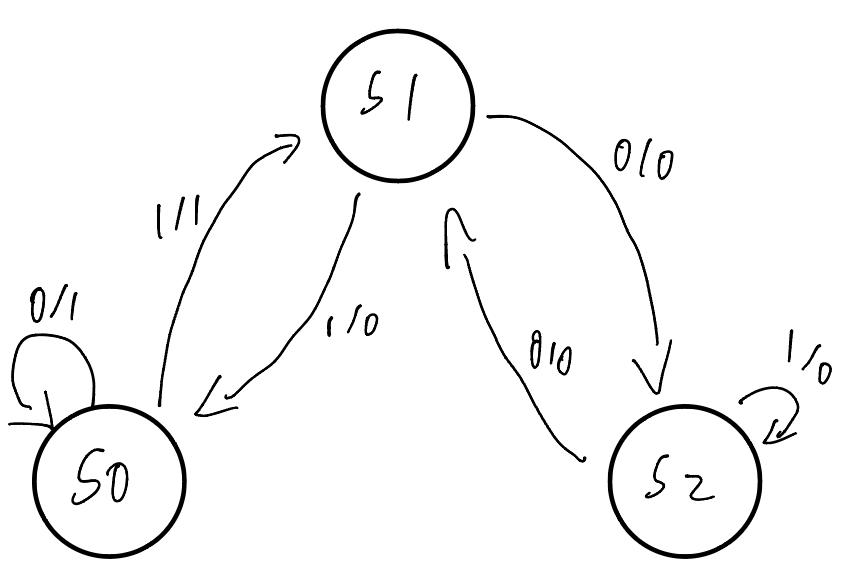
\includegraphics[scale=.38]{images/state_diagram.jpeg}
\subsection*{next\_stage\_logic:}
\begin{lstlisting}[language=Python]
def next_state_logic():
    next_state.next[0] = 
    (b & ~state[0] & ~state[1])|(~b & ~state[0] & state[1])
    next_state.next[1] = 
    (~b & state[0] & ~state[1])|(b & ~state[0] & state[1])
\end{lstlisting}

\subsection*{output\_logic:}
\begin{lstlisting}[language=Python]
def output_logic():
    z.next = 1 if state[1] == 0 and state[0] == 0 else 0
\end{lstlisting}

\subsection*{Out for 111000101}
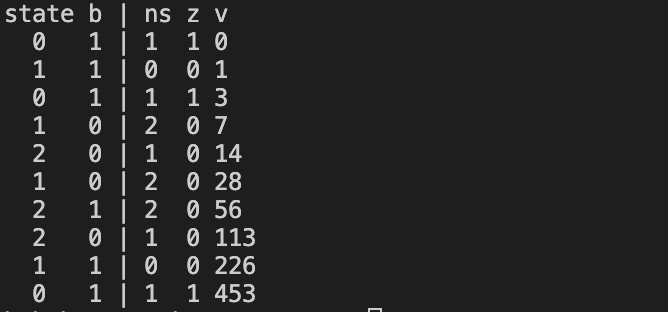
\includegraphics[scale=1]{images/Q1Out.png}

\section*{Problem 2}

Consider the multiplier we have studied. Inside the control module, there is also a register
that counts the steps and a combinational circuit. Assume the following. 
\begin{itemize}
    \item The delay of the adder is 10 ns, 
    \item The delay of the combinational circuit in the control module is 2 ns. 
    \item The setup time, the hold time, and the propagation delay of the registers is 0.5 ns, 0.2 ns,
    and 1 ns, respectively. 
    \item Do not consider the delays on wire.
\end{itemize}
Answer the following questions. Round answers to the nearest tenth if necessary. For
example, enter 3 for 3, 0.3 for 1/3, and 0.7 for 2/3. 
\subsection*{a.}
In a figure like below, show the timing of the following events.
\begin{enumerate}
    \item a1. Reg-Ready. The output of registers is available. 
    \item a2. Control-Ready. The output of control module is available
    \item a3. Adder-Ready. The output of adder is available.
    \item a4. Latest. The input to registers must be ready. This is the example in the figure.
\end{enumerate}

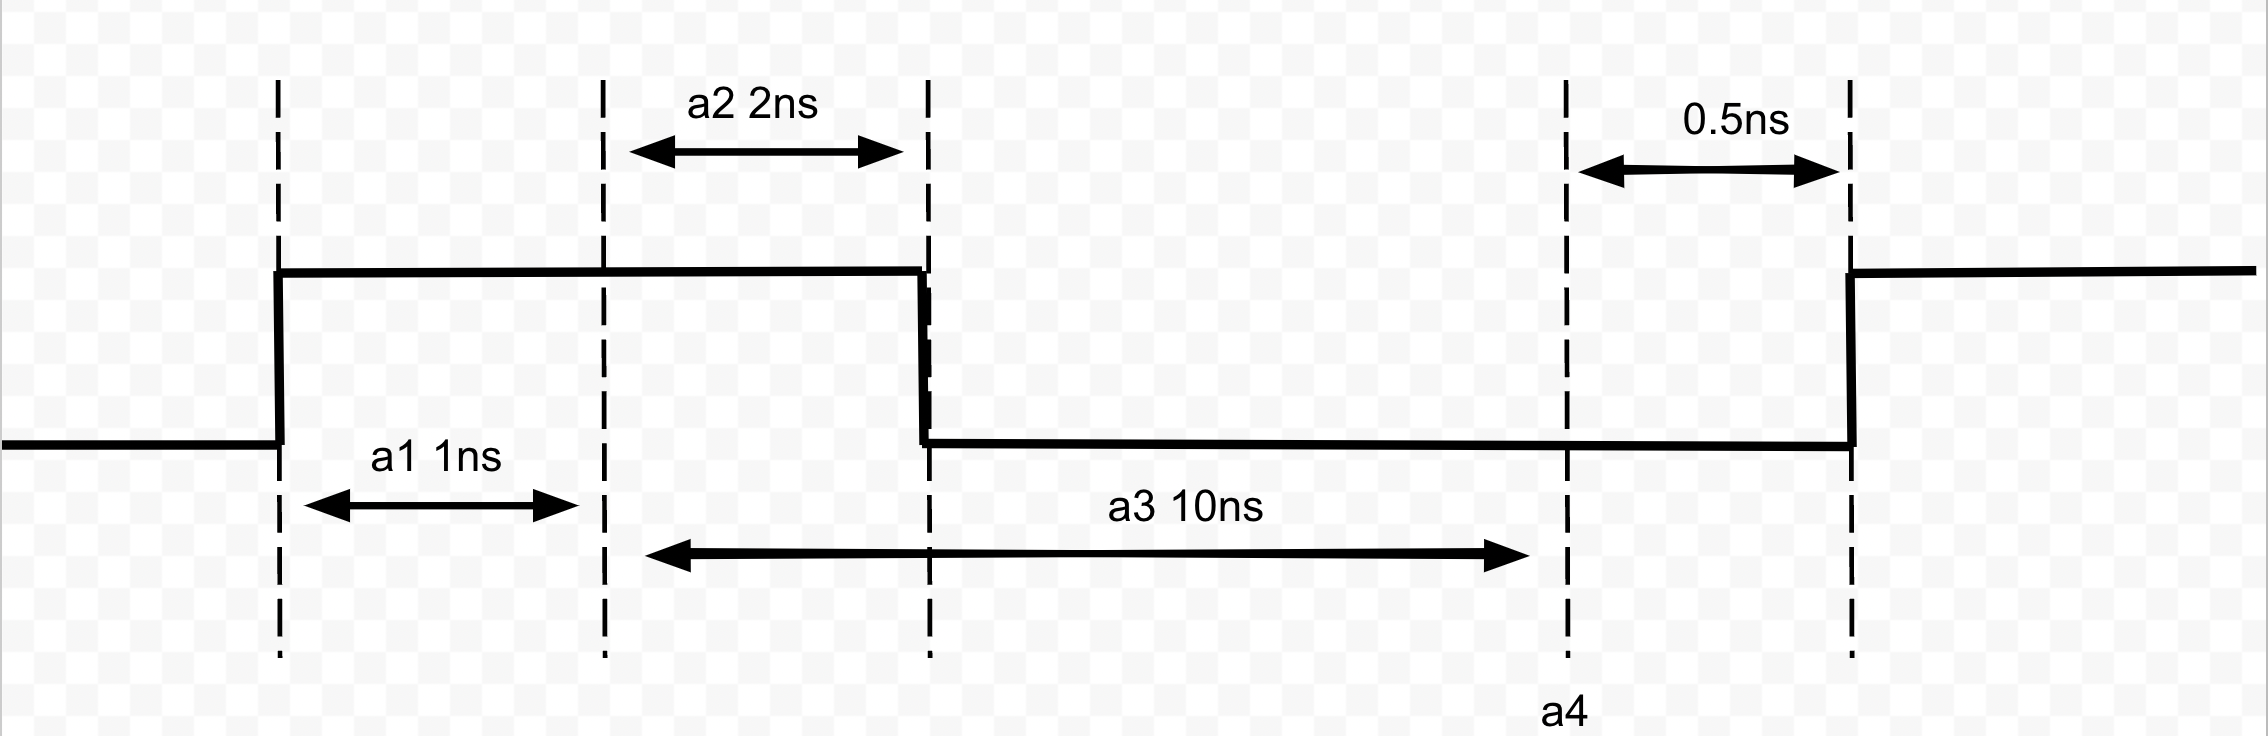
\includegraphics[scale=.29]{images/Q2.png}

\subsection*{b.}
What is the minimum cycle time for this multiplier to work properly?

The minimum cycle time is 10 ns + 1 ns + 0.5 ns = 11.5 ns.

\subsection*{c.}
What is the highest clock rate in MHz that this multiplier can run at?

The highest clock rate is 1/11.5 ns * 1000 = 86.96 MHz or 87 MHz.


\subsection*{d.}
If we build sequential circuit with the same kind of registers, what is the highest clock
rate in MHz we can achieve?

The highest clock rate is 1 ns + 0.5 ns = 1.5 ns. The highest clock rate is 1/1.5 ns * 1000 = 666.67 MHz or 667 MHz.





\section*{Problem 3}
\subsection*{Multiplier:}
\begin{table}[h]
    \resizebox{\textwidth}{!}{%
    \begin{tabular}{|l|l|l|l|}
    \hline
    Steps & Multiplicand & Multiplier & Product     \\ \hline
    init  & 00000 11011  & 10001      & 00000 00000 \\ \hline
    1     & 00001 10110  & 01000      & 00000 11011 \\ \hline
    2     & 00011 01100  & 00100      & 00000 11011 \\ \hline
    3     & 00110 11000  & 00010      & 00000 11011 \\ \hline
    4     & 01101 10000  & 00001      & 00000 11011 \\ \hline
    5     & 11011 00000  & 00000      & 01110 01011 \\ \hline
    \end{tabular}%
    }
\end{table}
01110 01011 = 459
27 * 17 = 459
Same value if consider unsigned
\section*{Problem 4}
Translate the following C function to RISC-V assembly code.
\begin{lstlisting}
char * uint2decstr(char s[], unsigned int v)
{
    unsigned int r;

    if (v >= 10) {
        s = uint2decstr(s, v / 10);
    }
    r = v % 10; // remainder
    s[0] = '0' + r;
    s[1] = 0;
    return &s[1]; // return the address of s[1]
}
\end{lstlisting}

\subsection*{Solution:}
\begin{lstlisting}
#       CSE 3666 uint2decstr

.globl  main

.data

str:	.space 128

    .text
main:   
# set all bytes in the buffer to 'A'
la	s1, str
    addi    a1, x0, 0
addi	a2, x1, 128
li	t2, 'A'
clear:
    add     t0, s1, a1
sb	t1, 0(t0)
    addi    a1, a1, 1
bne	a1, a2, clear

    addi    a0, s1, 0
    # change -1 to other numbers to test
    li	a1, 2022
jal	ra, uint2decstr

    addi    a0, s1, 0
    addi    a7, x0, 4
    ecall

exit:   addi    a7, x0, 10      
    ecall

# char * uint2decstr(char *s, unsigned int v) 
# the function converts unsigned value to decimal string
# Here are some examples:
# 0:    "0"
# 2022: "2022"
# -1:   "4294967295"

uint2decstr:
addi sp, sp, -8 # reserve space for return address and v
sw ra, 4(sp) # save return address
sw a1, 0(sp) # save v
addi t0, x0, 10 # t0 = 10
bltu a1, t0, cont # if v < 10 skips to cont
divu a1, a1, t0 # v = v / 10
jal ra, uint2decstr # call uint2decstr(s, v / 10)
cont:
lw ra, 4(sp) # restore return address
lw a1, 0(sp) # restore v
addi t0, x0, 10 # t0 = 10
remu t1, a1, t0 # t0 = v % 10
addi t0, t1, '0' # Set t0 to charcter of t1
sb t0, 0(a0) # s[0] = '0' + t1
sb t0, 1(a0) # s[1] = 0
addi a0, a0, 1 # a0 = &s[1]
addi sp, sp, 8 # free space
jr ra # return
\end{lstlisting}

\end{document}